\apendice{Planificación}

\section{Introducción}
En el desarrollo de este proyecto, utilizaremos la metodología SCRUM, con un desarrollo incremental con una duración de 2 semanas por Sprint. 
La organización en GitHub se realizará del siguiente modo: 
\begin{itemize}
\item Creación de un nuevo Milestone con una duración de 2 semanas el día de la reunión. 
\item Creación de los issues básicos necesarios para dicho Milestone. 
\item Desarrollo de los issues y la creación de los nuevos issues necesarios. 
\item Utilización de la herramienta Zenhub para el seguimiento de las tareas. 
\item Cierre de las issues una vez finalizadas para observar el avance de las tareas de forma real frente al progreso ideal. 
\end{itemize}

\section{Planificación temporal}
La evolución bisemanal de las tareas se ha realizado de la siguiente manera: 
\subsection{\textbf{Sprint 1}  (15/01/2018-29/01/2018) }
El primer Sprint, orientado hacia la explicación del desarrollo del proyecto. Se decidirán las herramientas básicas de la gestión de tareas, documentación de memoria y anexos y las referencias bibliográficas. 
Por ello: 
\begin{itemize}
\item Se ha documentado y probado la utilización de \LaTeX como editor de texto.
\item Se han documentado y probado los gestores de versiones de metodología ágil. 
\begin{itemize}
\item GitHub
\item Bitbucket
\end{itemize}
\item Se ha elegido la herramienta para la utilización de referencias bibliográficas. 
\begin{itemize}
\item BibTex
\item Zotero
\end{itemize}
\end{itemize}
\textbf{Problemáticas encontradas}\\En el primer Sprint, ante la falta de experiencia de la utilización de forma fluida de GitHub, consideramos ``Estimate'' de las issues como la dificultad de la tarea, por lo que, aun habiendo tareas más largas-principalmente documentación- pero más sencillas, consideramos dichas tareas con un nivel bajo en Estimate. Este problema persistirá en los 3 primeros Sprint, habiéndose corregido en el cuarto Sprint. La siguiente imagen corresponde al Burndown del Sprint 1~\ref{fig:A.2.1}
\begin{figure}[h]
\centering
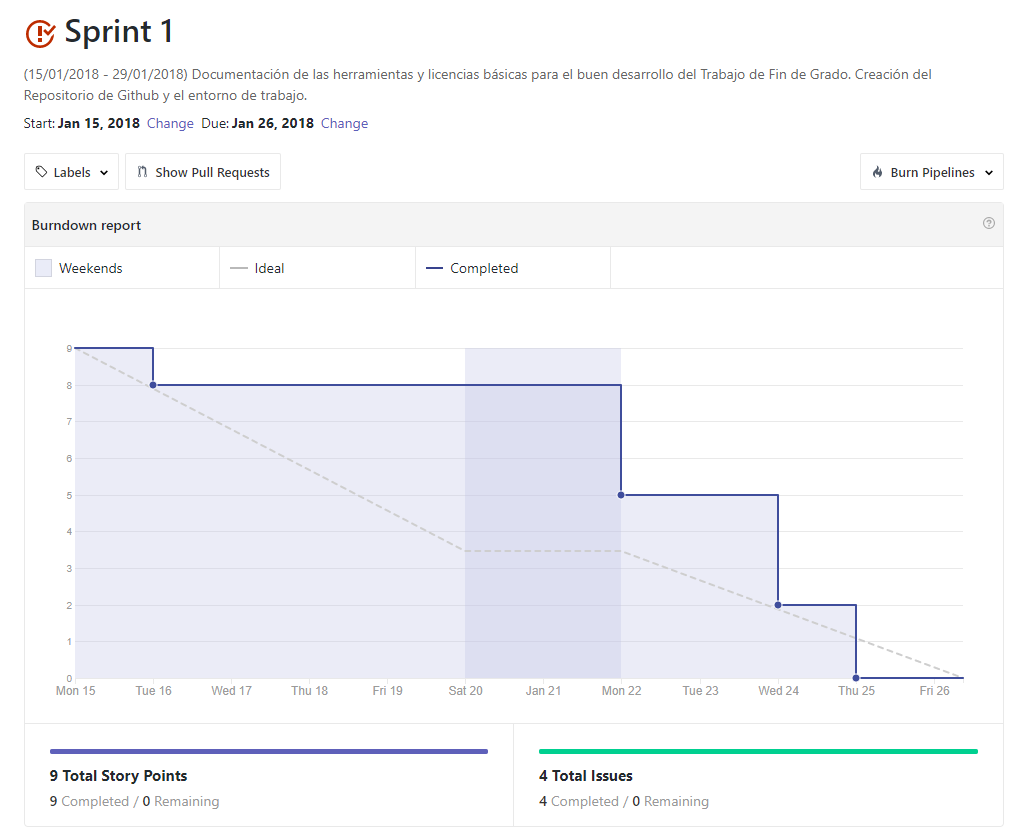
\includegraphics[width=0.90\textwidth]{Sprint_1}
\caption{Burndown del primer Sprint}
\label{fig:A.2.1}
\end{figure}

\subsection{\textbf{Sprint 2}  (29/01/2018-12/02/2018) }
El segundo Sprint, orientado hacia las técnicas utilizadas en \LaTeX así como las diferentes asígnaturas existentes en el Grado de Ingeniería Informática. Durante la reunión, se decidirá el tipo de cuestionario a realizar, y cómo orientarlo hacia la recogida de datos.  
Por ello: 
\begin{itemize}
\item Se ha comenzado el desarrollo de la Memoria en \LaTeX  y la documentación del mismo. 
\item Se han documentado las diferentes asignaturas existentes. 
\end{itemize}
\textbf{Problemáticas encontradas}\\En el segundo Sprint,hemos tenido el mismo problema que en el Sprint 1, teniendo en cuenta los ``Estimate'' como la dificultad, sin tener en cuenta que algunas tareas, a pesar de ser sencillas, tienen una mayor duración de tiempo. \\Además, nos hemos encontrado con menor tiempo, por lo que hemos tenido que traspasar un Issue al Sprint 3. \\Finalmente, hubo una confusión en el ``Due Date'', ya que habíamos considerado como el tiempo de comienzo en lugar del tiempo de fin. Dicho error fue corregido en el Sprint 3. \\La siguiente imagen corresponde al Burndown del Sprint 2~\ref{fig:A.2.2}
\begin{figure}[h]
\centering
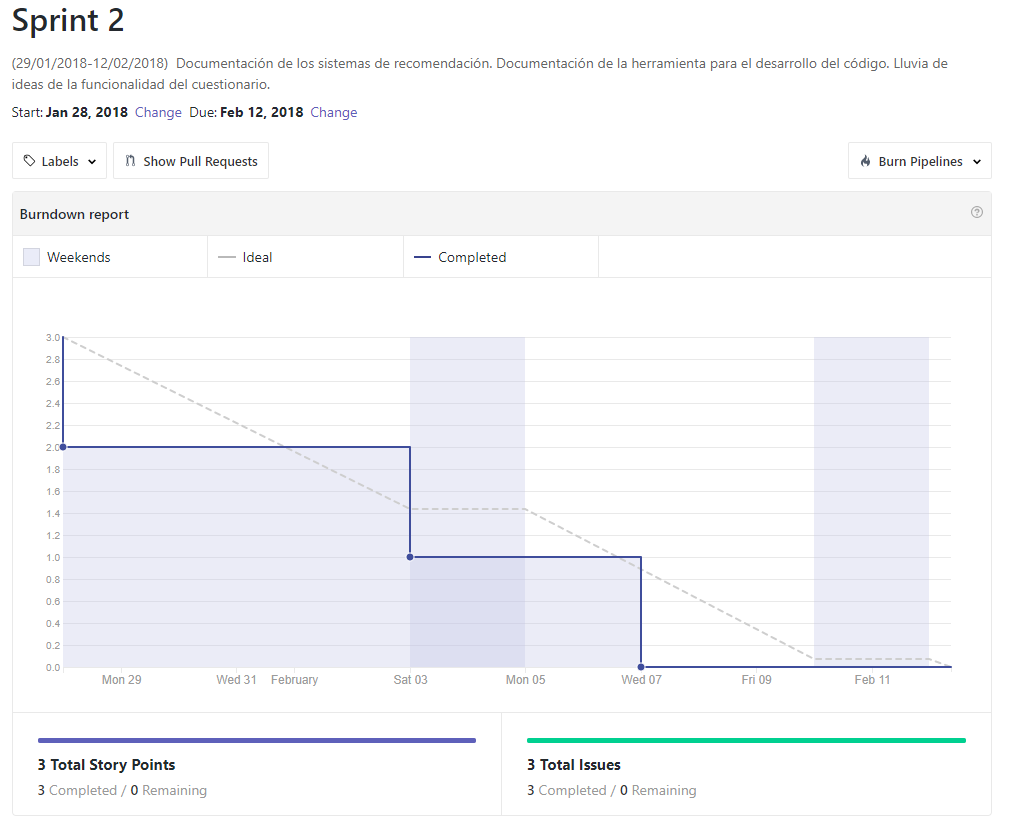
\includegraphics[width=0.90\textwidth]{Sprint_2}
\caption{Burndown del segundo Sprint}
\label{fig:A.2.2}
\end{figure}
\\

\subsection{\textbf{Sprint 3}  (13/02/2018-27/02/2018) }
El tercer Sprint, se ha orientado hacia la terminación del Sprint 2, ya que, por falta de tiempo, no se terminaron las issues. 
Por ello: 
\begin{itemize}
\item Se ha creado el formulario y distribuido entre los diferentes ex-alumnos del Grado de Ingeniería Informática en Burgos. 
\item Se ha documentado la metodología de integración de las funcionalidades del cuestionario y cómo almacenar los datos. 
\item Se ha realizado una documentación de los diferentes sistemas de Recomendación existentes.  
\end{itemize}
\textbf{Problemáticas encontradas}\\En el tercer Sprint,hemos tenido el mismo problema que en el Sprint 1 y 2, teniendo en cuenta los ``Estimate'' como la dificultad, sin tener en cuenta la duración del mismo.\\Por otro lado, al igual que en el Sprint 1 y el Sprint 2, no cerramos correctamente el Milestone, de forma que fue cerrado una vez comenzado el Sprint 4, a pesar de que las Issues se encontraban ya cerradas. \\La siguiente imagen corresponde al Burndown del Sprint 3~\ref{fig:A.2.3}
\begin{figure}[h]
\centering
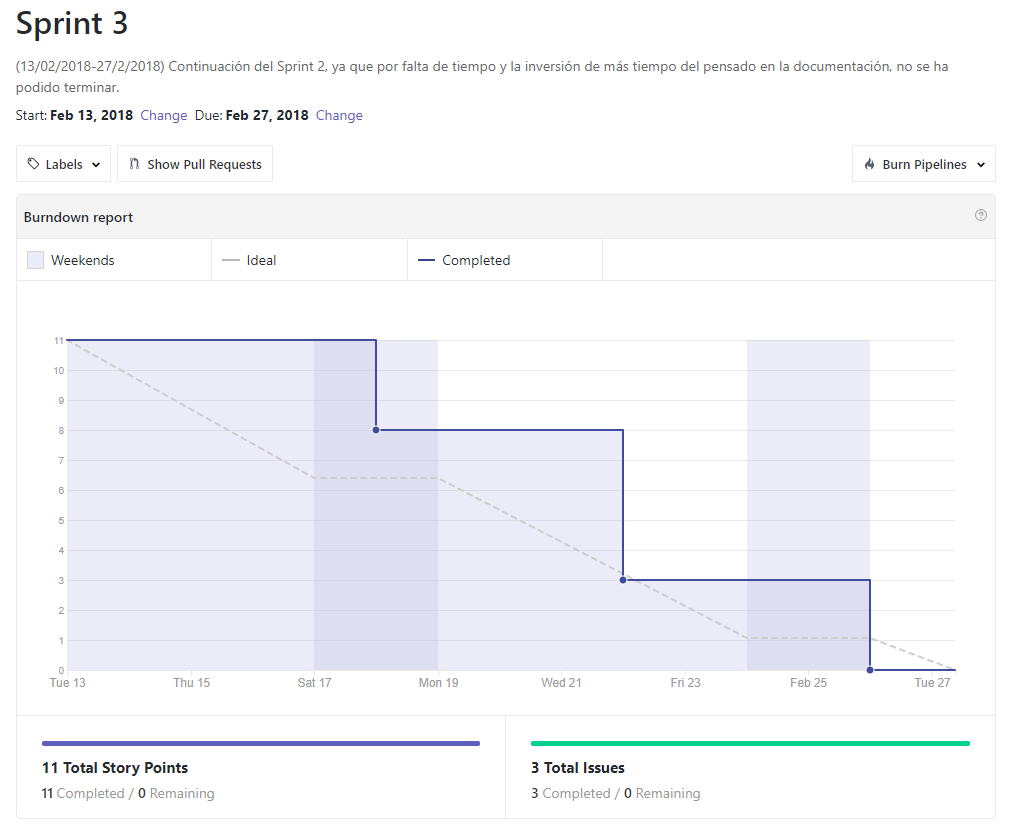
\includegraphics[width=0.90\textwidth]{Sprint_3}
\caption{Burndown del tercer Sprint}
\label{fig:A.2.3}
\end{figure}
\\

\subsection{\textbf{Sprint 4} (28/02/2018-14/03/2018) }
El cuarto  Sprint, se ha orientado hacia la integración de los resultados del cuestionario anónimo en Python, así como el desarrollo y corrección de memorias y anexos. 
Por ello: 
\begin{itemize}
\item Se han corregido las memorias y anexos, centrándonos en los errores ortográficos existentes.  
\item Se han creado las tablas explicativas de las memorias y anexos. 
\item Se ha documentado acerca de la API existente para sincronizar de forma dinámica los datos de Google Drive sin necesidad de descargar el fichero Excel. Para ello, se ha escogido la herramienta API GOOGLE-DIVE. 
\item Se ha desarrollado el código de integración de los datos-recogidos en el cuestionario- en Python.   
\end{itemize}
\textbf{Problemáticas encontradas}\\En el cuarto Sprint,tras sincronizar los datos del Excel con la API, y descargar el fichero json, hemos visto que los datos en Python no se sincronizan automáticamente, sino que se debe sincronizar manualmente de forma previa a la ejecución del código. Sin embargo, al ser el Admin quien se encarga de dicha tarea, no se considera un problema incompatible con la idea inicial del proyecto.  
 \\La siguiente imagen corresponde al Burndown del Sprint 4~\ref{fig:A.2.4}
\begin{figure}[h]
\centering
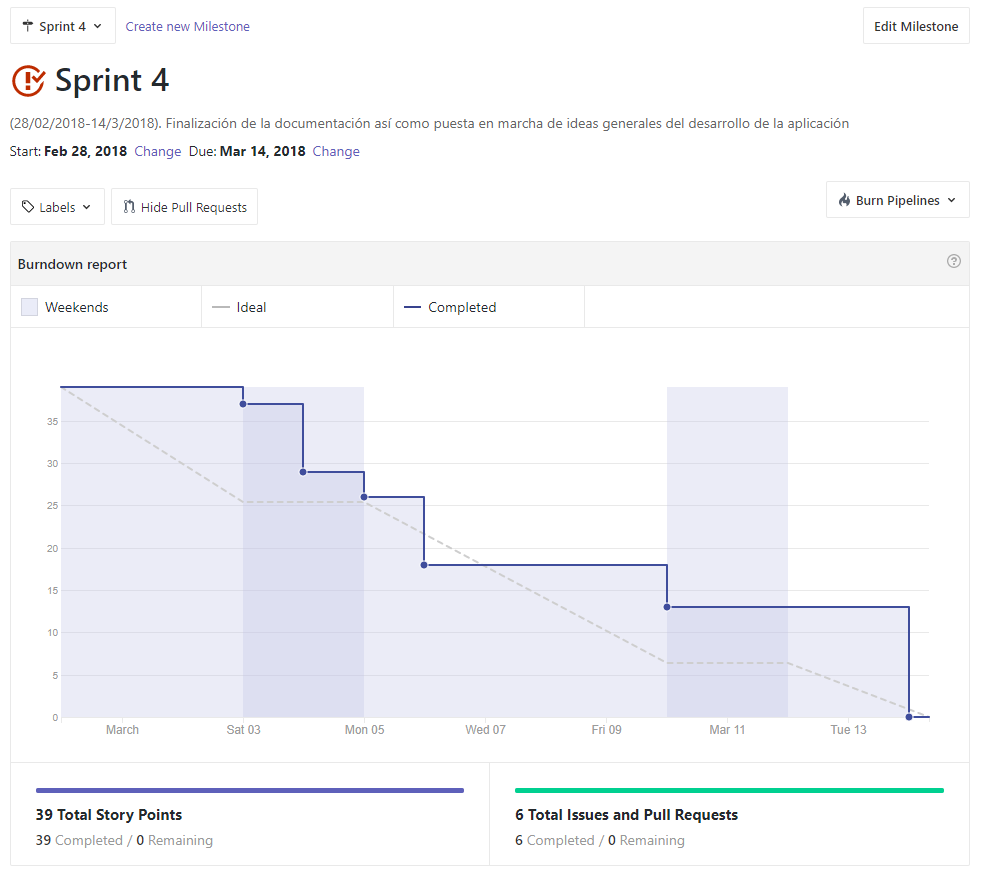
\includegraphics[width=0.90\textwidth]{Sprint_4}
\caption{Burndown del cuarto Sprint}
\label{fig:A.2.4}
\end{figure}
\\

\subsection{\textbf{Sprint 5} (15/03/2018-28/03/2018) }
El quinto  Sprint, se ha orientado hacia la documentación y el desarrollo del sistema de recomendación basado en productos. 
Por ello: 
\begin{itemize}
\item Se ha documentado el modo de diseño de la interfaz gráfica y probado su funcionamiento.   
\item Se ha desarrollado el sistema de recomendación basado en productos.  
\item Se ha desarrollado el plan de proyecto del Sprint 4.
 
\end{itemize}
\textbf{Problemáticas encontradas}\\En el quinto Sprint,nos hemos encontrado con la problemática de la dificultad del desarrollo del sistema de recomendación basado en productos de forma que no fuese necesario repetir diferentes funciones, simplificándolo, de forma que los métodos sean compatibles tanto  para el sistema de recomendación basado en usuarios como con el sistema de recomendación basado en productos. 
 \\La siguiente imagen corresponde al Burndown del Sprint 5~\ref{fig:A.2.5}
\begin{figure}[h]
\centering
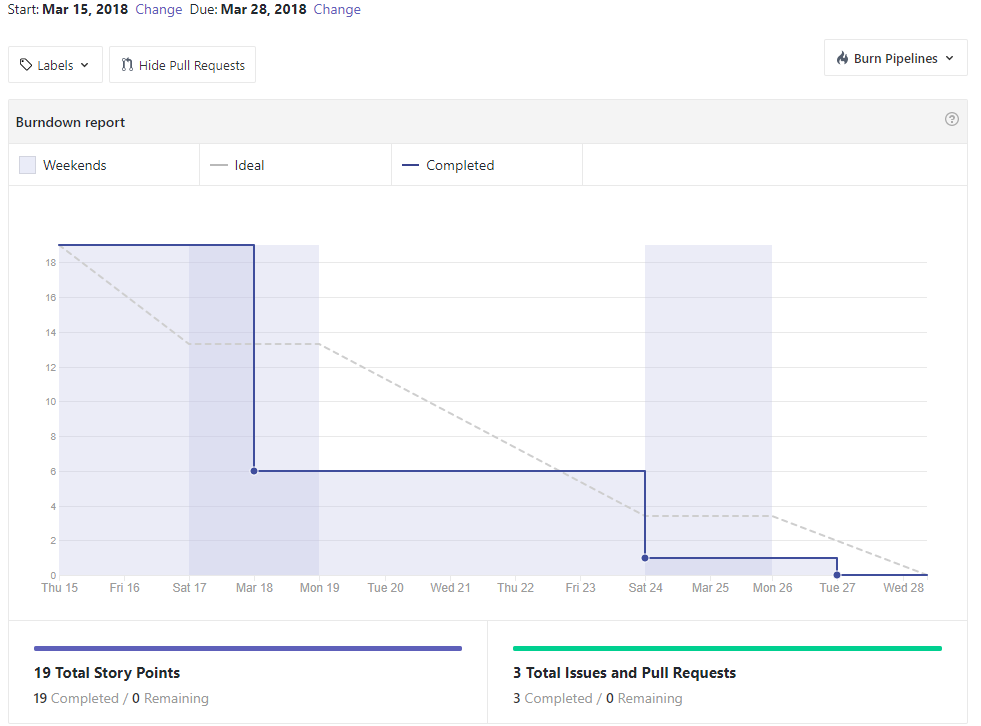
\includegraphics[width=0.90\textwidth]{Sprint_5}
\caption{Burndown del quinto Sprint}
\label{fig:A.2.5}
\end{figure}
\\

\subsection{\textbf{Sprint 6} (29/03/2018-12/04/2018) }
El sexto  Sprint, se ha orientado hacia la documentación, el desarrollo  y corrección de  diferentes sistemas de recomendación, así como la documentación del modo de almacenamiento de la información de los usuarios y asignaturas en cloud.  
Por ello: 
\begin{itemize}
\item Se ha documentado del sistema de recomendación basado en modeloSe ha documentado del modo de almacenamiento de los datos de los usuarios en cloud. 
\item Se ha continuado con el desarrollo de memorias y anexos. 
\item Se ha corregido el sistema de recomendación basado en productos. 
\item Se ha desarrollado el código del sistema de recomendación basado en usuarios.  

\end{itemize}
\textbf{Problemáticas encontradas}\\En el sexto Sprint,nos hemos encontrado con la problemática de cómo poder almacenar los datos de los usuarios de forma que se pudiese validar el usuario y contraseña, con un API que fuese gratuito. Por otra parte, hemos observado que hay un límite de llamadas al API que accede a  los datos almacenados en Google Drive. Esto no es un impedimento en el acceso a los mismos, ya que, al almacenar los datos en un fichero binario tras la carga, no es necesario realizar la llamada en cada ejecución del sistema de recomendación. 
 \\La siguiente imagen corresponde al Burndown del Sprint 6~\ref{fig:A.2.6}
\begin{figure}[h]
\centering
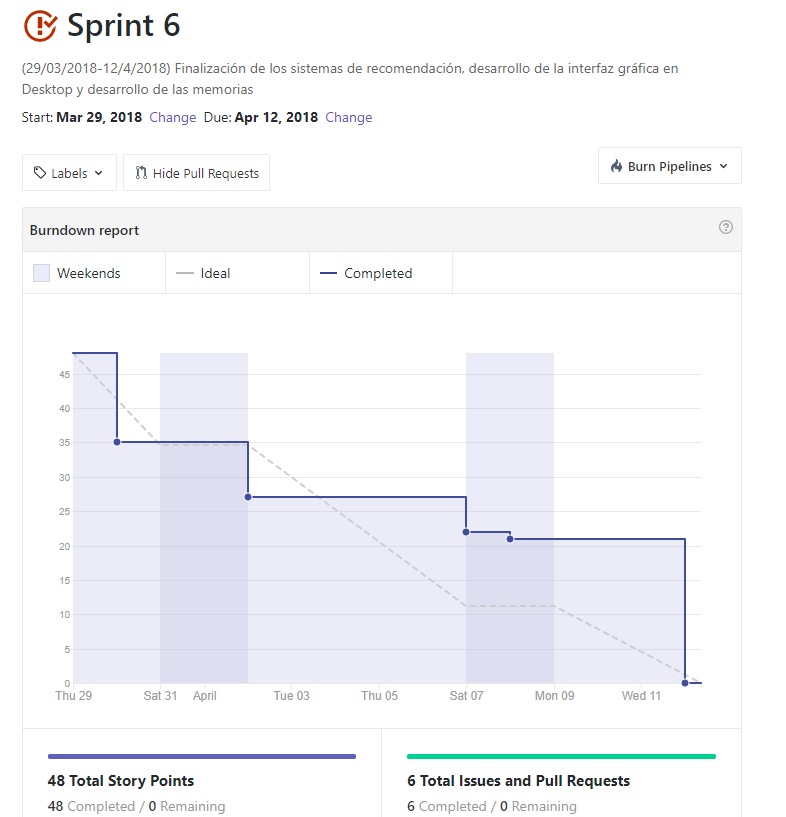
\includegraphics[width=0.90\textwidth]{Sprint_6}
\caption{Burndown del sexto Sprint}
\label{fig:A.2.6}
\end{figure}
\\



\subsection{\textbf{Sprint 7} (13/04/2018-27/04/2018) }
El séptimo  Sprint, se ha orientado hacia la documentación y  el desarrollo de memorias y anexos, así como la adaptación de los notebooks para ser utilizados en Eclipse utilizando el IDE de Python, PyDev. 
Por ello: 
\begin{itemize}
\item Se ha decidido la herramienta de desarrollo del proyecto. 
\item Se ha continuado con el desarrollo de memorias y anexos. 
\item Se ha desarrollado el plan de proyecto del Sprint 6.
\item Se ha adaptado el código de los notebooks en diferentes clases. 

\end{itemize}
\textbf{Problemáticas encontradas}\\En el Sprint 7, se continuó el desarrollo del sistema de recomendación basado en modelo, sin embargo, habiendo finalizado el Sprint, no se terminó con el código, por lo que se transpasó al  siguiente Sprint. 
 \\La siguiente imagen corresponde al Burndown del Sprint 7~\ref{fig:A.2.7}
\begin{figure}[h]
\centering
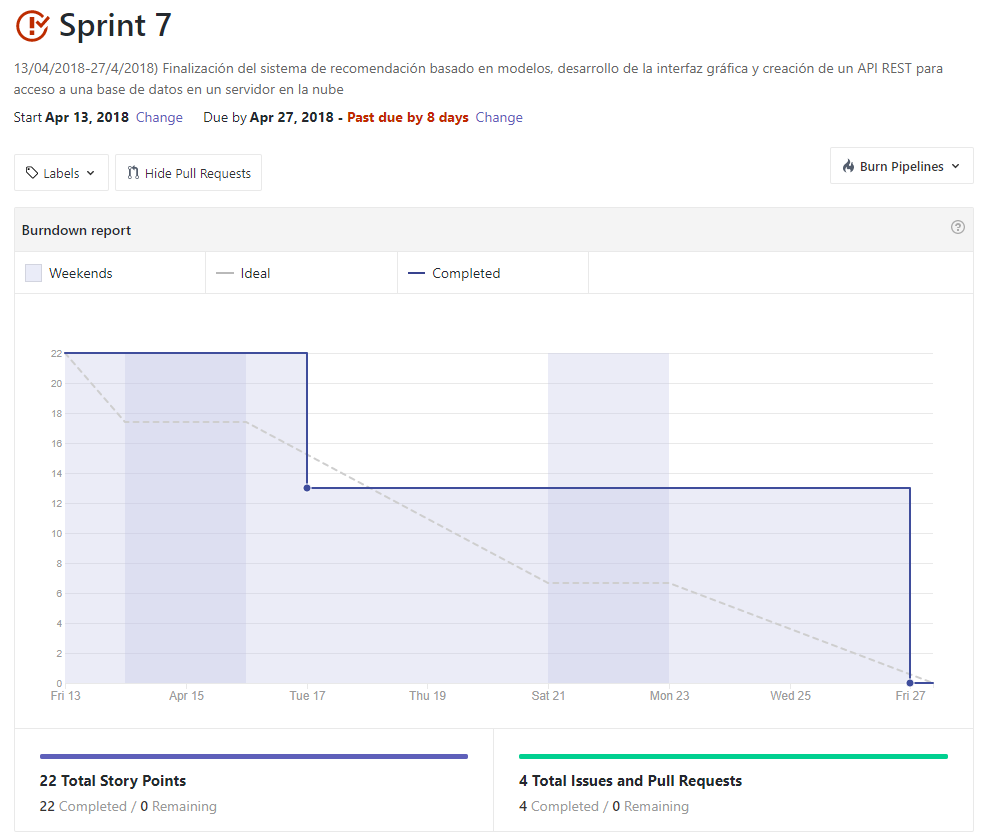
\includegraphics[width=0.90\textwidth]{Sprint_7}
\caption{Burndown del séptimo Sprint}
\label{fig:A.2.7}
\end{figure}
\\

\subsection{\textbf{Sprint 8} (28/04/2018-12/05/2018) }
El octavo  Sprint, se ha orientado hacia el desarrollo de memorias y anexos, tablas explicativas de las asignaturas para el desarrollo de posteriores gráficas, así como el desarrollo del sistema de recomendación basado en modelos. 
Por ello: 
\begin{itemize}
\item Se ha desarrollado el código del sistema de recomendación basado en modelos. 
\item Se ha continuado con el desarrollo de memorias y anexos. 
\item Se ha desarrollado el plan de proyecto del Sprint 7.
\item Se han creado las Entity necesarias (Usuarios  y Asignatura). 
\item Se ha creado en Excel la tabla explicativa del contenido general de las asignaturas. 
\end{itemize}
\textbf{Problemáticas encontradas}\\En el Sprint 8, se comenzó el desarrollo de los Requisitos Funcionales, a pesar de no haberse podido terminar, así como la adaptación a \LaTeX de la misma. Por otro lado, se comenzó el diseño de una posible interfaz gráfica versión 1.0, no habiéndose finalizado. \\Otra problemática encontrada ha sido un bug en el código del sistema de recomendación basado en modelos que aun no ha sido corregido. 
 \\La siguiente imagen corresponde al Burndown del Sprint 8~\ref{fig:A.2.8}
\begin{figure}[h]
\centering
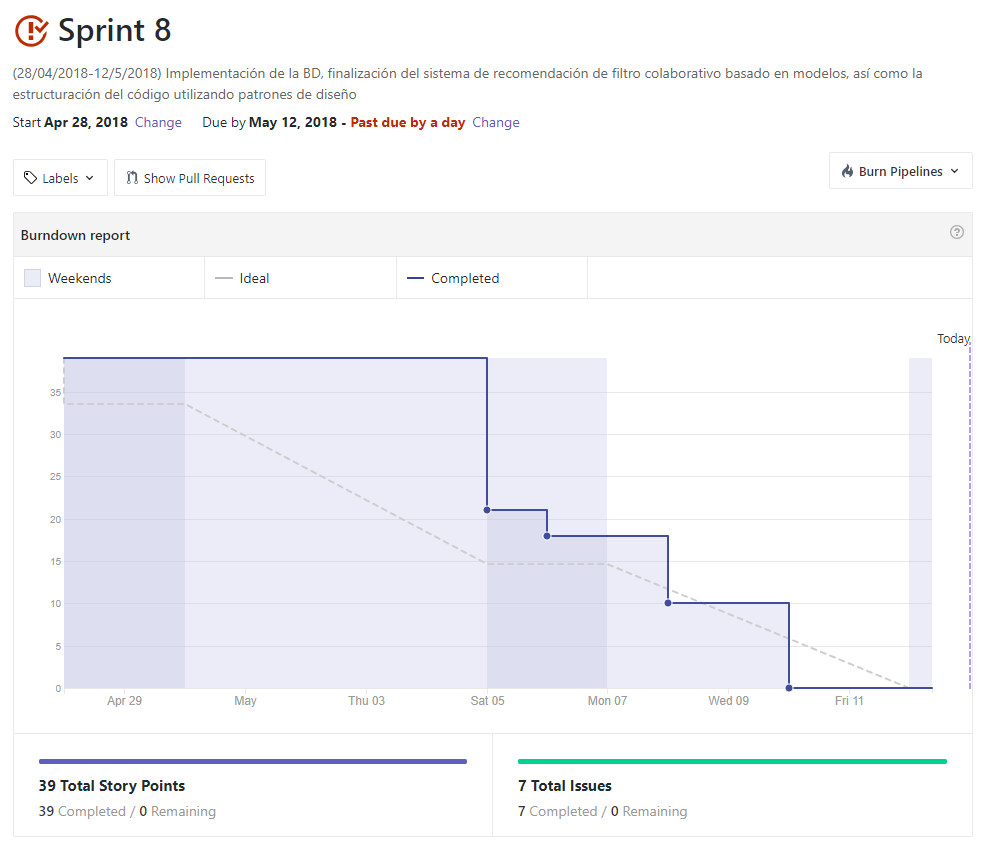
\includegraphics[width=0.90\textwidth]{Sprint_8}
\caption{Burndown del octavo Sprint}
\label{fig:A.2.8}
\end{figure}
\\
